\documentclass[tikz, border=20pt]{standalone}
\usepackage{amsmath, amssymb}
\usetikzlibrary{decorations.pathreplacing}

\begin{document}
	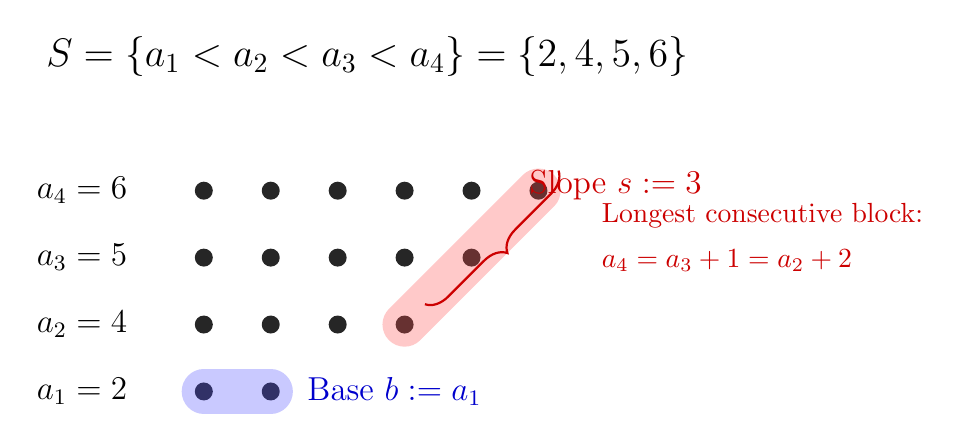
\begin{tikzpicture}[
		scale=0.85,
		dot/.style={circle, fill=black!85, minimum size=6.5pt, inner sep=0pt},
		highlight base/.style={blue!70, line width=16pt, opacity=0.3, line cap=round},
		highlight slope/.style={red!70, line width=16pt, opacity=0.3, line cap=round}
		]
		
		% Title / Set Definition
		\node[anchor=west, font=\Large] at (-1.5, 6) {$S = \{a_1 < a_2 < a_3 < a_4\} = \{2, 4, 5, 6\}$};
		
		% Draw dots and row labels corresponding to the elements of S
		\foreach \y/\n/\label in {4/6/a_4, 3/5/a_3, 2/4/a_2, 1/2/a_1} {
			% Draw row label
			\node[left, font=\large] at (0, \y) {$\label = \n$};
			
			% Draw dots
			\foreach \x in {1,...,\n} {
				\node[dot] at (\x, \y) {};
			}
		}
		
		% Highlight Base
		\draw[highlight base] (1,1) -- (2,1);
		\node[blue!80!black, right, font=\large] at (2.4, 1) {Base $b := a_1$};
		
		% Highlight Slope
		\draw[highlight slope] (6,4) -- (4,2);
		
		% Brace for Slope
		\draw[decorate, decoration={brace, amplitude=8pt}, thick, red!80!black] 
		(6.3, 4.3) -- (4.3, 2.3) 
		node[midway, above right=10pt, align=left, font=\large] {Slope $s := 3$};
		
		% Text for slope definition
		\node[anchor=west, red!80!black, align=left] at (6.8, 3.3) {
			Longest consecutive block:\\[4pt]
			$a_4 = a_3+1 = a_2+2$
		};
		
	\end{tikzpicture}
\end{document}